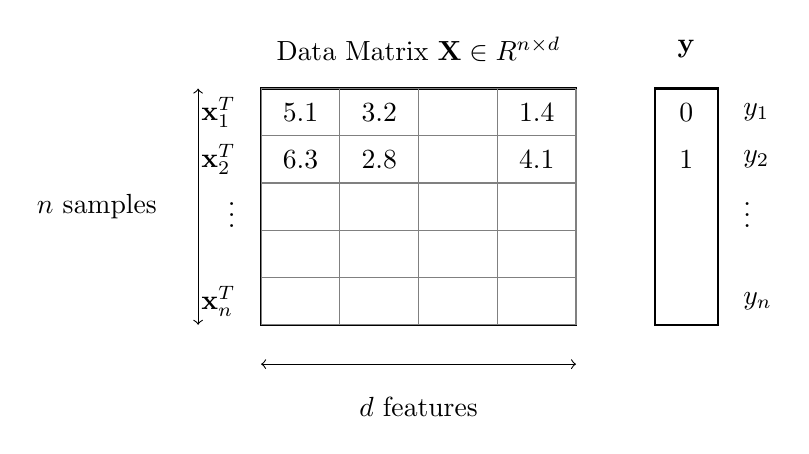
\begin{tikzpicture}[scale=1.0]
  % Dataset matrix X
  \draw[thick] (0,0) rectangle (4,3);
  \node at (2, 3.5) {Data Matrix $\mathbf{X} \in \mathbb{R}^{n \times d}$};
  
  % Grid lines
  \foreach \i in {0,1,2,3,4} {
    \draw[thin, gray] (\i, 0) -- (\i, 3);
  }
  \foreach \i in {0,0.6,1.2,1.8,2.4,3} {
    \draw[thin, gray] (0, \i) -- (4, \i);
  }
  
  % Row labels (samples)
  \node[left] at (-0.2, 2.7) {$\mathbf{x}_1^T$};
  \node[left] at (-0.2, 2.1) {$\mathbf{x}_2^T$};
  \node[left] at (-0.2, 1.5) {$\vdots$};
  \node[left] at (-0.2, 0.3) {$\mathbf{x}_n^T$};
  
  % % Column labels (features)
  % \node[above] at (0.5, 3.2) {$x^{(1)}$};
  % \node[above] at (1.5, 3.2) {$x^{(2)}$};
  % \node[above] at (2.5, 3.2) {$\cdots$};
  % \node[above] at (3.5, 3.2) {$x^{(d)}$};
  
  % Target vector y
  \draw[thick] (5,0) rectangle (5.8,3);
  \node at (5.4, 3.5) {$\mathbf{y}$};
  
  \node[right] at (6, 2.7) {$y_1$};
  \node[right] at (6, 2.1) {$y_2$};
  \node[right] at (6, 1.5) {$\vdots$};
  \node[right] at (6, 0.3) {$y_n$};
  
  % Annotations
  \draw[<->] (-0.8, 0) -- (-0.8, 3);
  \node[left] at (-1.2, 1.5) {$n$ samples};
  
  \draw[<->] (0, -0.5) -- (4, -0.5);
  \node[below] at (2, -0.8) {$d$ features};
  
  % Example values
  \node at (0.5, 2.7) {$5.1$};
  \node at (1.5, 2.7) {$3.2$};
  \node at (3.5, 2.7) {$1.4$};
  \node at (5.4, 2.7) {$0$};
  
  \node at (0.5, 2.1) {$6.3$};
  \node at (1.5, 2.1) {$2.8$};
  \node at (3.5, 2.1) {$4.1$};
  \node at (5.4, 2.1) {$1$};
\end{tikzpicture}
